%!TEX root=../main.tex
\section{Results}
\label{sec:love_results}

In this section we demonstrate the effectiveness and speed of LOVE{}, both at computing predictive variances and also at posterior sampling.
%Our goal is to show that 1) LOVE{} produces uncertainties and samples that are indistinguishable from the state-of-the-art, and 2) that LOVE{} offers substantial speed improvements.
All LOVE{} variances are computed with $k=50$ Lanczos iterations,
and KISS-GP models use $m\!=\!10,\!000$ inducing points unless otherwise stated.
We perform experiments using the GPyTorch library.\footnote{
  \url{github.com/cornellius-gp/gpytorch}}
We optimize models with ADAM \cite{kingma2014adam} and a learning rate of $0.1$.
All timing experiments utilize GPU acceleration, performed on a NVIDIA GTX 1070.

\subsection{Predictive Variances}
\label{sec:results_variances}

We measure the accuracy and speed of LOVE + KISS-GP{} at computing predictive variances.
We compare variances computed with a LOVE + KISS-GP{} model against variances computed with an Exact GP ({\bf Exact}).
On datasets that are too large to run exact GP inference, we instead compare the LOVE + KISS-GP{} variances against KISS-GP variances computed in the standard way ({\bf KISS-GP w/o LOVE{}}).
\citet{wilson2015thoughts} show that KISS-GP variances recover the exact variance up to 4 decimal places.
Therefore, we will know that LOVE + KISS-GP{} produces accurate variances if it matches standard KISS-GP w/o LOVE{}.
We report the scaled mean absolute error (SMAE)\footnote{
  Mean absolute error divided by the variance of y.
} \cite{rasmussen2006gaussian} of LOVE{} variances compared against these baselines.
%(Note that the predictive posterior means are \emph{completely identical} with both methods, as LOVE{} only affects variance calculations.)
For each dataset, we optimize the hyperparameters of a KISS-GP model.
We then use the same hyperparameters for each baseline model when computing variances.

\begin{figure}[t!]
  \centering
  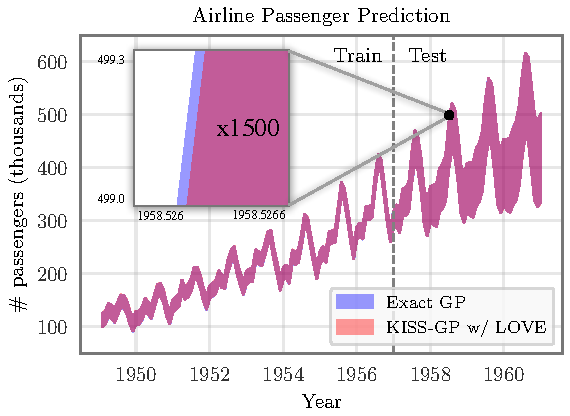
\includegraphics[width=0.70\columnwidth]{figures/airline_comparison.pdf}
  \caption[Comparison of LOVE predictive variances verses exact predictive variances on airline passenger extrapolation.]{
    Comparison of LOVE predictive variances verses exact predictive variances on airline passenger extrapolation.
    The LOVE{} variances are accurate within $10^{-4}$.
    \label{fig:airline_results}
  }
\end{figure}

\paragraph{One-dimensional example.}
We first demonstrate LOVE{} on a complex one-dimensional regression task.
The airline passenger dataset ({\bf Airline}) measures the average monthly number of passengers from 1949 to 1961 \cite{hyndman2005time}.
We aim to extrapolate the numbers for the final 4 years (48 measurements) given data for the first 8 years (96 measurements).
%These data exhibit short-term periodic trends as well as long-term growth trends.  Consequentially,
Accurate extrapolation on this dataset requires a kernel function capable of expressing various patterns, such as the spectral mixture (SM) kernel \cite{wilson2013gaussian}.
Our goal is to evaluate if LOVE{} produces reliable predictive variances, even with complex kernel functions.

We compute the variances for Exact GP, KISS-GP w/o LOVE{}, and KISS-GP + LOVE{} models with a $10$-mixture SM kernel.
In \cref{fig:airline_results}, we see that the LOVE + KISS-GP{} confidence intervals match the Exact GP's intervals extremely well.
The SMAE of LOVE{}'s predicted variances (compared against Exact GP variances) is $1.29 \times 10^{-4}$.
Although not shown in the plot, we confirm the reliability of these predictions by computing the log-likelihood of the test data.
We compare the LOVE + KISS-GP{} model to an Exact GP, a KISS-GP model without LOVE{}, and a sparse variational GP (SGPR) model with $m=1000$ inducing points.\footnote{
 Implemented in GPFlow \cite{matthews2017gpflow}} \cite{titsias2009variational,hensman2013gaussian}.
All methods achieve nearly identical log-likelihoods, ranging from $-221$ to $-222$.


\begin{table}[t!]
  \caption[Speedup and accuracy of LOVE + KISS-GP{} for predictive variances.]{
    Speedup and accuracy of LOVE + KISS-GP{} for predictive variances.
    KISS-GP and Exact GPs use deep kernel learning.
    Speed results are measured on GPUs.
    Accuracy is measured by Scaled Mean Average Error.
    ($N$ is the number of data, $D$ is the dimensionality.)
    \label{tab:large_dataset_results}
  }
  \vspace{0.5ex}
  \centering
  \resizebox{\textwidth}{!}{%
    %!TEX root=../main.tex
\begin{tabular}{ |ccc||c|c||c|c| }
  \hline
  \multicolumn{3}{|c|}{\bf Dataset}
  & \multicolumn{4}{c|}{\thead{\bf Variance SMAE}}
  \\
  \cline{1-7}
  Name
  & {$N$}
  & {$D$}
  & {\thead{(vs KISS-GP w/o LOVE)}}
  & {\thead{(vs Exact GP)}}
  & {\thead{(from scratch)}}
  & {\thead{(after pre-comp.)}}
  \\
  \hhline{|===#=|=#=|=|}
  \thead{\bf Airfoil}
  & $1,\!503$
  & $6$
  & $1.30 \times 10^{-5}$
  & $7.01 \times 10^{-5}$
  & $4 \times$
  & $84 \times$
  %& $3 \times$
  %& $49 \times$
  %& $9 \times$
  %& $183 \times$
  \\

  \thead{\bf Skillcraft}
  & $3,\!338$
  & $19$
  & $2.00 \times 10^{-7}$
  & $2.86 \times 10^{-4}$
  & $25 \times$
  & $167 \times$
  %& $4 \times$
  %& $70 \times$
  %& $17 \times$
  %& $110 \times$
  \\

  \thead{\bf Parkinsons}
  & $5,\!875$
  & $20$
  & $8.80 \times 10^{-5}$
  & $5.18 \times 10^{-3}$
  & $46 \times$
  & $443 \times$
  %& $3 \times$
  %& $33 \times$
  %& $16 \times$
  %& $152 \times$
  \\

  \thead{\bf PoleTele}
  & $15,\!000$
  & $26$
  & $2.90 \times 10^{-5}$
  & $1.08 \times 10^{-3}$
  & $78 \times$
  & $1178 \times$
  %& $1.5 \times$
  %& $40 \times$
  %& $21 \times$
  %& $343 \times$
  \\

  \thead{\bf Elevators}
  & $16,\!599$
  & $18$
  & $1.20 \times 10^{-6}$
  & --
  & $64 \times$
  & $1017 \times$
  %& $2 \times$
  %& $31 \times$
  %& $20 \times$
  %& $316 \times$
  \\

  \thead{\bf Kin40k}
  & $40,\!000$
  & $8$
  & $3.90 \times 10^{-7}$
  & --
  & $31 \times$
  & $2065 \times$
  %& $8 \times$
  %& $81 \times$
  %& $12 \times$
  %& $798 \times$
  \\

  \thead{\bf Protein}
  & $45,\!730$
  & $9$
  & $5.30 \times 10^{-5}$
  & --
  & $44 \times$
  & $1151 \times$
  %& $10 \times$
  %& $109 \times$
  %& $20 \times$
  %& $520 \times$
  \\
  \hline
\end{tabular}

  }
  \vspace{1em}

  \resizebox{\textwidth}{!}{%
    %!TEX root=../main.tex
\begin{tabular}{ |ccc||c|c|c|c| }
  \hline
  \multicolumn{3}{|c||}{\bf Dataset}
  & \multicolumn{4}{c|}{\thead{\bf Speedup over SGPR}}
  \\
  \cline{1-7}
  \multirow{2}{*}{Name}
  & \multirow{2}{*}{$N$}
  & \multirow{2}{*}{$D$}
  & \thead{(from scratch)}
  & \thead{(after pre-comp.)}
  & \thead{(from scratch)}
  & \thead{(after pre-comp.)}
  \\
   &  &  & $M=100$ & $M=100$ & $M=1000$ & $M=1000$
  \\
  \hhline{|===#=|=|=|=|}
  \thead{\bf Airfoil}
  & $1,\!503$
  & $6$
  %& $1.30 \times 10^{-5}$
  %& $7.01 \times 10^{-5}$
  %& $4 \times$
  %& $84 \times$
  & $3 \times$
  & $49 \times$
  & $9 \times$
  & $183 \times$
  \\

  \thead{\bf Skillcraft}
  & $3,\!338$
  & $19$
  %& $2.00 \times 10^{-7}$
  %& $2.86 \times 10^{-4}$
  %& $25 \times$
  %& $167 \times$
  & $4 \times$
  & $70 \times$
  & $17 \times$
  & $110 \times$
  \\

  \thead{\bf Parkinsons}
  & $5,\!875$
  & $20$
  %& $8.80 \times 10^{-5}$
  %& $5.18 \times 10^{-3}$
  %& $46 \times$
  %& $443 \times$
  & $3 \times$
  & $33 \times$
  & $16 \times$
  & $152 \times$
  \\

  \thead{\bf PoleTele}
  & $15,\!000$
  & $26$
  %& $2.90 \times 10^{-5}$
  %& $1.08 \times 10^{-3}$
  %& $78 \times$
  %& $1178 \times$
  & $1.5 \times$
  & $40 \times$
  & $21 \times$
  & $343 \times$
  \\

  \thead{\bf Elevators}
  & $16,\!599$
  & $18$
  %& $1.20 \times 10^{-6}$
  %& --
  %& $64 \times$
  %& $1017 \times$
  & $2 \times$
  & $31 \times$
  & $20 \times$
  & $316 \times$
  \\

  \thead{\bf Kin40k}
  & $40,\!000$
  & $8$
  %& $3.90 \times 10^{-7}$
  %& --
  %& $31 \times$
  %& $2065 \times$
  & $8 \times$
  & $81 \times$
  & $12 \times$
  & $798 \times$
  \\

  \thead{\bf Protein}
  & $45,\!730$
  & $9$
  %& $5.30 \times 10^{-5}$
  %& --
  %& $44 \times$
  %& $1151 \times$
  & $10 \times$
  & $109 \times$
  & $20 \times$
  & $520 \times$
  \\
  \hline
\end{tabular}

  }
\end{table}

\paragraph{Large datasets.}
We measure the accuracy of LOVE{} variances on several large-scale regression benchmarks from the UCI repository \cite{asuncion2007uci}.
We compute the variance for all test set data points.
Each of the models use deep RBF kernels (DKL) on these datasets with the architectures described in \cite{wilson2016deep}.
Deep RBF kernels are extremely flexible (with up to $10^5$ hyperparameters) and are well suited to model many types of functions.
In \cref{tab:large_dataset_results}, we report the SMAE of the LOVE + KISS-GP{} variances compared against the two baselines.
On all datasets, we find that LOVE{} matches KISS-GP w/o LOVE{} variances to at least $5$ decimal points.
Furthermore, LOVE + KISS-GP{} is able to approximate Exact variances with no more than than $0.1\%$ average error.
For any given test point, the maximum variance error is similarly small (e.g. $\leq \! 2.6\%$ on Skillcraft and $\leq \! 2.0\%$ on PoleTele).
Therefore, using LOVE{} to compute variances results in \emph{almost no loss in accuracy}.

\paragraph{Speedup.}
In \cref{tab:large_dataset_results} we compare the variance computation speed of a KISS-GP model with and without LOVE{} on the UCI datasets.
In addition, we compare against the speed of SGPR with a standard RBF kernel, a competitive scalable GP approach.
On all datasets, we measure the time to compute variances {\bf from scratch}, which includes the cost of pre-computation (though, as stated in \cref{sec:love_method}, this typically occurs during training).
In addition, we report the speed {\bf after pre-computing} any terms that aren't specific to test points (which corresponds to the test time speed).
We see in \cref{tab:large_dataset_results} that KISS-GP + LOVE{} yields a substantial speedup over KISS-GP without LOVE{}.
The speedup is between $4\times$ and $44\times$, even when accounting for LOVE{}'s precomputation.
At test time after pre-computation, LOVE{} is \emph{up to $2,\!000\times$ faster}.
Additionally, LOVE + KISS-GP{} is significantly faster than SGPR models.
For SGPR models with $m=100$ inducing points, the LOVE + KISS-GP{} model (with $m=10,\!000$ inducing points) is up to $10\times$ faster before pre-computation and $100\times$ faster after.
With $m=1000$ SGPR models, LOVE + KISS-GP{} is up to $20\times$/$500\times$ faster before/after precomputation.
The biggest improvements are obtained on the largest datasets since LOVE{}, unlike other methods, is independent of dataset size at test time.

\begin{figure}[t!]
  \centering
  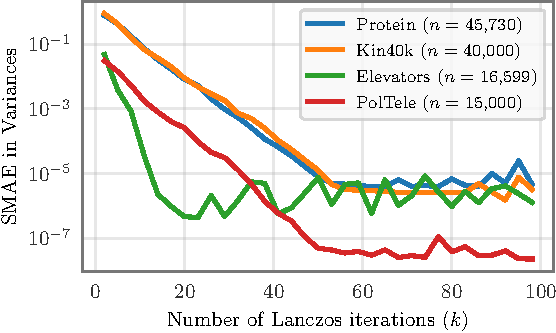
\includegraphics[width=0.70\columnwidth]{figures/lanczos_accuracy.pdf}
  \vspace{-2ex}
  \caption[LOVE variance error verses number of Lanczos iterations.]{
    LOVE variance error verses number of Lanczos iterations
    (KISS-GP model, $M=10,\!000$. Protein, Kin40k, PoleTele, and Elevators UCI datasets).
    \label{fig:lanczos_accuracy}
  }
  \vspace{-1ex}
\end{figure}

\paragraph{Accuracy vs. Lanczos iterations.}
In \cref{fig:lanczos_accuracy}, we measure the accuracy of LOVE{} as a function of the number of Lanczos iterations ($k$).
We train a KISS-GP model with a deep RBF kernel on the four largest datasets from \cref{tab:large_dataset_results}, using the setup described above.
We measure the SMAE of LOVE + KISS-GP's predictive variances compared against the standard KISS-GP variances (KISS-GP w/o LOVE).
As seen in \cref{fig:lanczos_accuracy}, error decreases \emph{exponentially} with the number of Lanczos iterations, up until roughly $50$ iterations.
After roughly $50$ iterations, the error levels off, though this may be an artifact of floating-point precision (which may also cause small subsequent fluctuations).
Recall that $J$ also corresponds with the rank of the $\bR$ matrices in \cref{eqn:pred_covar_ski_fast}.



\subsection{Sampling}

\begin{table}[t!]
  \caption[Accuracy and computation time of drawing samples from the predictive distribution.]{
    Accuracy and computation time of drawing samples from the predictive distribution.
    \label{tab:sampling_results}
  }
  \vspace{0.5ex}
  \centering
  \resizebox{\textwidth}{!}{%
    %!TEX root=../main.tex
\begin{tabular}{ |c||c|c|c|c|c| }
  \hline
  \multirow{4}{*}{\thead{\bf Dataset} }
  & \multicolumn{5}{c|}{\thead{\bf Sample Covariance Error} }

  \\
  \cline{2-6}


  & \thead{\bf Exact GP \\ \bf w/ Cholesky}
  & \thead{\bf Fourier \\ \bf Features}
  & \thead{\bf SGPR \\ ($M=100$)}
  & \thead{\bf SGPR \\ ($M=1000$)}
  & \thead{\bf LOVE \\ \bf + KISS-GP}
  %& \thead{\bf Fourier \\ \bf Features}
  %& \thead{\bf SGPR (m=100)}
  %& \thead{\bf SGPR (m=1000)}
  %& \thead{\bf KISS-GP \\ \bf w/ LOVE{} \\ (from scratch)}
  %& \thead{\bf KISS-GP \\ \bf w/ LOVE{} \\ (after pre-comp.)}
  \\
  \hhline{|=#=|=|=|=|=|}

  \thead{\bf PolTele}
  & $\mathbf{8.8 \times 10^{-4}}$
  & $1.8 \times 10^{-3}$
  & $4.9 \times 10^{-3}$
  & $2.7 \times 10^{-3}$
  & $\mathbf{7.5 \times 10^{-4}}$
  %& $22 \times$
  %& $24 \times$
  %& $3 \times$
  %& $21 \times$
  %& $\mathbf{881 \times}$
  \\

  \thead{\bf Elevators}
  & $\mathbf{2.6 \times 10^{-7}}$
  & $3.1 \times 10^{-4}$
  & $8.7 \times 10^{-6}$
  & $3.6 \times 10^{-6}$
  & $\mathbf{5.5 \times 10^{-7}}$
  %& $31 \times$
  %& $33 \times$
  %& $4 \times$
  %& $25 \times$
  %& $\mathbf{1062 \times}$
  \\
  \hline

  \thead{\bf BO (Eggholder)}
  & $\mathbf{7.7 \times 10^{-4}}$
  & $1.5 \times 10^{-3}$
  & $\mathbf{8.1 \times 10^{-4}}$
  & --
  & $\mathbf{8.0 \times 10^{-5}}$
  %& $16 \times$
  %& $8 \times$
  %& --
  %& $19 \times$
  %& $\mathbf{775 \times}$
  \\

  \thead{\bf BO (Styblinski-Tang)}
  & $\mathbf{5.4 \times 10^{-4}}$
  & $7.3 \times 10^{-3}$
  & $\mathbf{5.2 \times 10^{-4}}$
  & --
  & $\mathbf{5.2 \times 10^{-4}}$
  %& $11 \times$
  %& $8 \times$
  %& --
  %& $42 \times$
  %& $\mathbf{18,\!100 \times}$
  \\
  \hline

\end{tabular}

  }
  \vspace{1em}

  \resizebox{\textwidth}{!}{%
    %!TEX root=../main.tex
\begin{tabular}{ |c||c|c|c|c|c| }
  \hline
  \multirow{4}{*}{\thead{\bf Dataset} }
  & \multicolumn{5}{c|}{\thead{\bf Speedup over Exact GP w/ Cholesky} }

  \\
  \cline{2-6}


  %& \thead{\bf Exact GP \\ \bf w/ Cholesky}
  %& \thead{\bf Fourier \\ \bf Features}
  %& \thead{\bf SGPR (m=100)}
  %& \thead{\bf SGPR (m=1000)}
  %& \thead{\bf KISS-GP \\ \bf w/ LOVE}
  & \thead{\bf Fourier \\ \bf Features}
  & \thead{\bf SGPR \\ ($M=100$)}
  & \thead{\bf SGPR \\ ($M=1000$)}
  & \thead{\bf LOVE \\ \bf + KISS-GP{} \\ (from scratch)}
  & \thead{\bf LOVE \\ \bf + KISS-GP{} \\ (after pre-comp.)}
  \\
  \hhline{|=#=|=|=|=|=|}

  \thead{\bf PolTele}
  %& $\mathbf{8.8 \times 10^{-4}}$
  %& $1.8 \times 10^{-3}$
  %& $4.9 \times 10^{-3}$
  %& $2.7 \times 10^{-3}$
  %& $\mathbf{7.5 \times 10^{-4}}$
  & $22 \times$
  & $24 \times$
  & $3 \times$
  & $21 \times$
  & $\mathbf{881 \times}$
  \\

  \thead{\bf Elevators}
  %& $\mathbf{2.6 \times 10^{-7}}$
  %& $3.1 \times 10^{-4}$
  %& $8.7 \times 10^{-6}$
  %& $3.6 \times 10^{-6}$
  %& $\mathbf{5.5 \times 10^{-7}}$
  & $31 \times$
  & $33 \times$
  & $4 \times$
  & $25 \times$
  & $\mathbf{1062 \times}$
  \\
  \hline

  \thead{\bf BO (Eggholder)}
  %& $\mathbf{7.7 \times 10^{-4}}$
  %& $1.5 \times 10^{-3}$
  %& $\mathbf{8.1 \times 10^{-4}}$
  %& --
  %& $\mathbf{8.0 \times 10^{-5}}$
  & $16 \times$
  & $8 \times$
  & --
  & $19 \times$
  & $\mathbf{775 \times}$
  \\

  \thead{\bf BO (Styblinski-Tang)}
  %& $\mathbf{5.4 \times 10^{-4}}$
  %& $7.3 \times 10^{-3}$
  %& $\mathbf{5.2 \times 10^{-4}}$
  %& --
  %& $\mathbf{5.2 \times 10^{-4}}$
  & $11 \times$
  & $8 \times$
  & --
  & $42 \times$
  & $\mathbf{18,\!100 \times}$
  \\
  \hline

\end{tabular}

  }
\end{table}

We evaluate the quality of posterior samples drawn with LOVE + KISS-GP{} as described in \cref{sec:sampling_method}.
We compare these samples to three baselines: sampling from an {\bf Exact GP} using the Cholesky decomposition, sampling from an {\bf SGPR} model with Cholesky, and sampling with random {\bf Fourier features} \citep{rahimi2008random} -- a method commonly used in Bayesian optimization \cite{hernandez2014predictive,wang2017max}.
The LOVE + KISS-GP{} and SGPR models use the same architecture as described in the previous section.
For Fourier features, we use 5000 random features -- the maximum number of features that could be used without exhausting available GPU memory.
We learn hyperparameters on the Exact GP and then use the same hyperparameters for the all methods.

We test on the two largest UCI datasets which can still be solved exactly (PolTele, Eleveators) and two Bayesian optimization benchmark functions (Eggholder -- 2 dimensional, and Styblinski-Tang -- 10 dimensional).
The UCI datasets use the same training procedure as in the previous section.
For the BayesOpt functions, we evaluate the model after 100 queries of max value entropy search \cite{wang2017max}.
We use a standard (non-deep) RBF kernel for Eggholder, and for Syblinski-Tang we use the additive kernel decomposition suggested by~\citet{kandasamy2015high}.\footnote{
  The Syblinski-Tang KISS-GP model uses the sum of 10 RBF kernels -- one for each dimension -- and $m=100$ inducing points.
}

\paragraph{Sample accuracy.}
In \cref{tab:sampling_results} we evaluate the accuracy of the different sampling methods.
We draw $s\!=\!1000$ samples at $t\!=\!10,\!000$ test locations and compare the sample covariance matrix with the true posterior covariance matrix $k_{f\mid\dset}(\bXtest,\bXtest)$ in terms of element-wise mean absolute error.
It is worth noting that all methods incur some error -- even when sampling with an Exact GP.
Nevertheless, Exact GPs, SGPR, and LOVE{} produce very accurate sample covariance matrices.
In particular, Exact GPs and LOVE{} achieve between 1 and 3 orders of magnitude less error than the random Fourier Feature method.

\paragraph{Speed.}
Though LOVE{}, Exact GPs, and SGPR have similar sample accuracies, LOVE{} is much faster.
Even when accounting for LOVE's pre-computation time (i.e. sampling ``from scratch''), LOVE{} is comparable to Fourier features and SGPR in terms of speed.
At test time (i.e. after pre-computation), LOVE{} is up to $18,\!000$ times faster than Exact.

\paragraph{Bayesian optimization.}
Many acquisition functions in Bayesian optimization rely on sampling from the posterior GP.
For example, max-value entropy search \cite{wang2017max} draws samples from a posterior GP in order to estimate the function's maximum value $p(y^{*} \! \mid \! \dset)$.
The corresponding maximum \emph{location} distribution, $p(x^{*} \! \mid \! \dset)$, is also the primary distribution of interest in predictive entropy search \cite{hernandez2014predictive}.
%
\begin{figure}[t!]
  \centering
  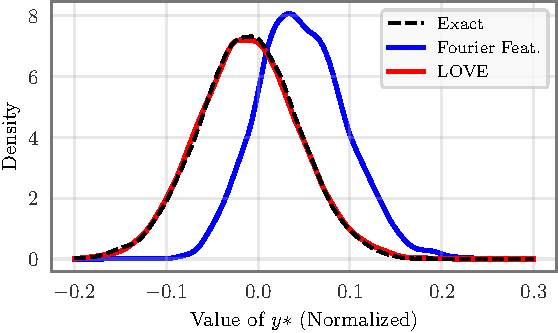
\includegraphics[width=0.70\columnwidth]{figures/thompson_sampling_comparison.pdf}
  \caption[Comparison of LOVE and Random Fourier Features for BayesOpt sampling.]{
    Comparison of LOVE and Random Fourier Features for BayesOpt sampling.
    Each line represents an approximation of maximum value distribution $p(y_\text{max} \mid \dset)$ using different sampling methods (exact sampling, Random Fourier Features, and LOVE + KISS-GP).
    Samples drawn with LOVE+KISSGP closely match samples drawn using an Exact GP.
    (Dataset: (normalized) Eggholder function after 100 iterations of BayesOpt.)
    \label{fig:thompson_sampling_comparison}
  }
    \vspace{-2ex}
\end{figure}
%
In \cref{fig:thompson_sampling_comparison}, we visualize each method's sampled distribution of $p(y^{*} \! \mid \! \dset)$ for the Eggholder benchmark.
We plot kernel density estimates of the sampled maximum value distributions after $100$ BayesOpt iterations.
Since the Exact GP sampling method uses the exact Cholesky decomposition, its sampled max-value distribution can be considered closest to ground truth.
The Fourier feature sampled distribution differs significantly.
In contrast, LOVE{}'s sampled distribution very closely resembles the Exact GP distribution, yet
LOVE{} is $700 \times$ faster than the Exact GP on this dataset (\cref{tab:sampling_results}).
